\subsection{Explicación general del diseño}
\par El modelo presentado se basa en un sistema de simulación que es configurado con los siguientes subsistemas:
\begin{itemize}
  \item \textbf{Sistema de construcción}: es el encargado de crear y almacenar los planes de construcción de pozos de extracción, plantas procesadoras y tanques de almacenamiento. También almacena los catálogos de plantas procesadoras y tanques de almacenamiento y gestiona las conexiones entre pozos de excavación, tanques de almacenamiento y plantas procesadoras.
  \item \textbf{Sistema de ejecución de criterios}: se encarga de llevar a cabo la ejecución de cada criterio del sistema.
  \item \textbf{Sistema de gestión de excavadoras}: posee el catálogo de excavadoras y gestiona su alquiler. También almacena el estado de las excavadoras alquiladas.
  \item \textbf{Sistema de gestión de parcelas}: Es quien conoce al yacimiento y administra las parcelas utilizadas y libres.
  \item \textbf{Sistema de extracción}: Es quien se encarga de crear los eventos de extracción y almacenarlos.
  \item \textbf{Criterios de simulación}: Es quien conoce a los criterios de distintos tipos. El simulador acude a él para conocer los criterios que debe ejecutar.
\end{itemize}

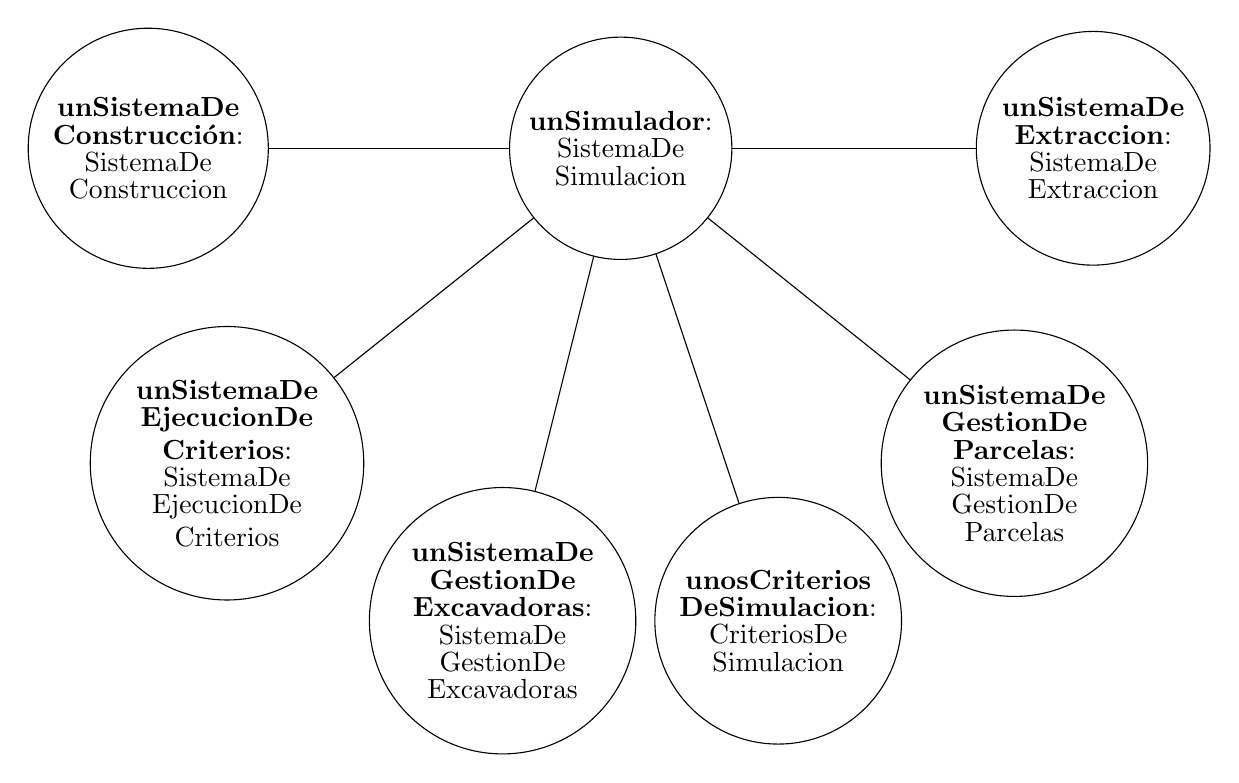
\begin{tikzpicture}
  \node[shape=circle,draw=black] (unSimulador) at (0,0) {\shortstack{\textbf{unSimulador}:\\SistemaDe\\Simulacion}};
  \node[shape=circle,draw=black] (unSistemaDeConstruccion) at (-6,0) {\shortstack{\textbf{unSistemaDe}\\\textbf{Construcción}:\\SistemaDe\\Construccion}};
  \node[shape=circle,draw=black] (unSistemaDeEjecucionDeCriterios) at (-5,-4) {\shortstack{\textbf{unSistemaDe}\\\textbf{EjecucionDe}\\\textbf{Criterios}:\\SistemaDe\\EjecucionDe\\Criterios}};
  \node[shape=circle,draw=black] (unSistemaDeGestionDeExcavadoras) at (-1.5,-6) {\shortstack{\textbf{unSistemaDe}\\\textbf{GestionDe}\\\textbf{Excavadoras}:\\SistemaDe\\GestionDe\\Excavadoras}};
  \node[shape=circle,draw=black] (unSistemaDeGestionDeParcelas) at (5,-4) {\shortstack{\textbf{unSistemaDe}\\\textbf{GestionDe}\\\textbf{Parcelas}:\\SistemaDe\\GestionDe\\Parcelas}};
  \node[shape=circle,draw=black] (unSistemaDeExtraccion) at (6,0) {\shortstack{\textbf{unSistemaDe}\\\textbf{Extraccion}:\\SistemaDe\\Extraccion}};
  \node[shape=circle,draw=black] (unosCriteriosDeSimulacion) at (2,-6) {\shortstack{\textbf{unosCriterios}\\\textbf{DeSimulacion}:\\CriteriosDe\\Simulacion}};

  \path [-] (unSimulador) edge node[left] {} (unSistemaDeConstruccion);
  \path [-] (unSimulador) edge node[left] {} (unSistemaDeEjecucionDeCriterios);
  \path [-] (unSimulador) edge node[left] {} (unSistemaDeGestionDeExcavadoras);
  \path [-] (unSimulador) edge node[left] {} (unSistemaDeGestionDeParcelas);
  \path [-] (unSimulador) edge node[left] {} (unSistemaDeExtraccion);
  \path [-] (unSimulador) edge node[left] {} (unosCriteriosDeSimulacion);
\end{tikzpicture}



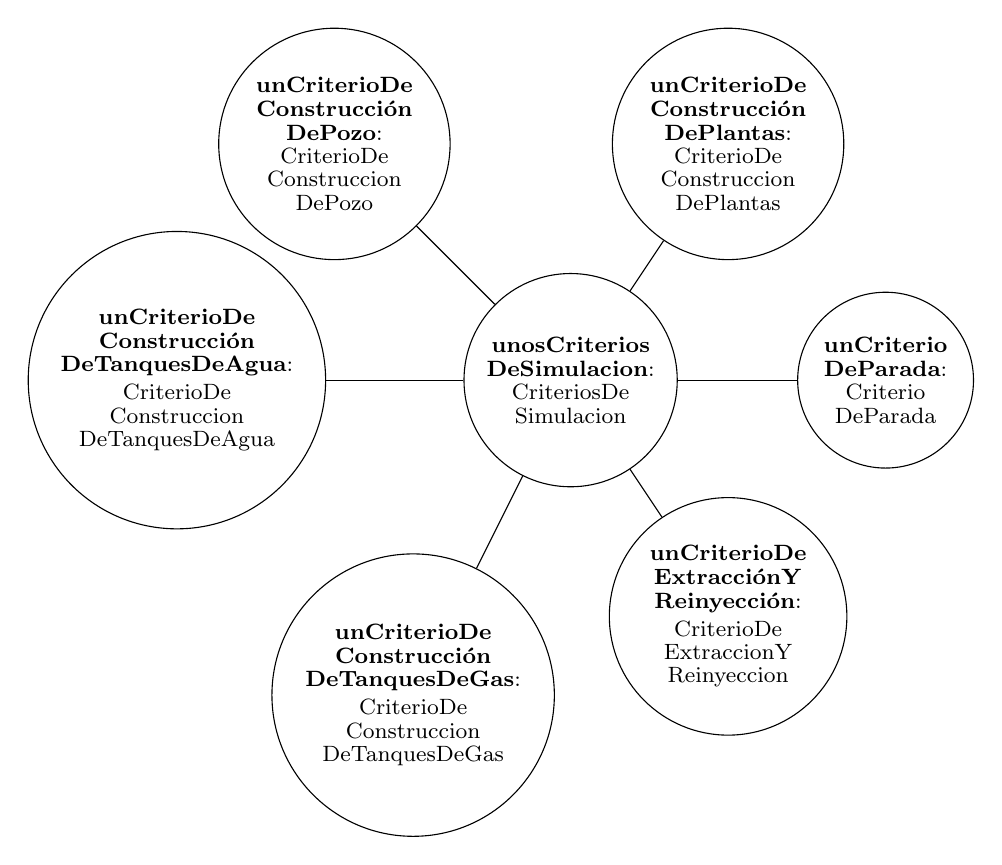
\begin{tikzpicture}
  \node[shape=circle,draw=black] (unosCriteriosDeSimulacion) at (0,0) {\footnotesize\shortstack{\textbf{unosCriterios}\\\textbf{DeSimulacion}:\\CriteriosDe\\Simulacion}};
  \node[shape=circle,draw=black] (unCriterioDeConstruccionDePozo) at (-3,3) {\footnotesize\shortstack{\textbf{unCriterioDe}\\\textbf{Construcción}\\\textbf{DePozo}:\\CriterioDe\\Construccion\\DePozo}};
  \node[shape=circle,draw=black] (unCriterioDeConstruccionDePlantas) at (2,3) {\footnotesize\shortstack{\textbf{unCriterioDe}\\\textbf{Construcción}\\\textbf{DePlantas}:\\CriterioDe\\Construccion\\DePlantas}};
  \node[shape=circle,draw=black] (unCriterioDeConstruccionDeTanquesDeAgua) at (-5,0) {\footnotesize\shortstack{\textbf{unCriterioDe}\\\textbf{Construcción}\\\textbf{DeTanquesDeAgua}:\\CriterioDe\\Construccion\\DeTanquesDeAgua}};
  \node[shape=circle,draw=black] (unCriterioDeConstruccionDeTanquesDeGas) at (-2,-4) {\footnotesize\shortstack{\textbf{unCriterioDe}\\\textbf{Construcción}\\\textbf{DeTanquesDeGas}:\\CriterioDe\\Construccion\\DeTanquesDeGas}};
  \node[shape=circle,draw=black] (unCriterioDeExtraccionYReinyeccion) at (2,-3) {\footnotesize\shortstack{\textbf{unCriterioDe}\\\textbf{ExtracciónY}\\\textbf{Reinyección}:\\CriterioDe\\ExtraccionY\\Reinyeccion}};
  \node[shape=circle,draw=black] (unCriterioDeParada) at (4,0) {\footnotesize\shortstack{\textbf{unCriterio}\\\textbf{DeParada}:\\Criterio\\DeParada}};

  \path [-] (unosCriteriosDeSimulacion) edge node[left] {} (unCriterioDeConstruccionDePozo);
  \path [-] (unosCriteriosDeSimulacion) edge node[left] {} (unCriterioDeConstruccionDePlantas);
  \path [-] (unosCriteriosDeSimulacion) edge node[left] {} (unCriterioDeConstruccionDeTanquesDeAgua);
  \path [-] (unosCriteriosDeSimulacion) edge node[left] {} (unCriterioDeConstruccionDeTanquesDeGas);
  \path [-] (unosCriteriosDeSimulacion) edge node[left] {} (unCriterioDeExtraccionYReinyeccion);
  \path [-] (unosCriteriosDeSimulacion) edge node[left] {} (unCriterioDeParada);
\end{tikzpicture}
